\documentclass[main.tex]{subfiles}
\begin{document}
\setcounter{section}{1}

\section{Installation and Getting Started}\label{sec:installation}

\subsection{Prerequisites}
{\it Smooth Emulator} software should run on UNIX, Mac OS or Linux, but is not supported for Windows OS. {\it Smooth Emulator} is largely  written in C++. In addition to a C++ compiler, the user needs the following software installed.

\begin{itemize}
    \item git
    \item CMake
    \item Eigen3 (Linear Algebra Package)
    \item GSL (Gnu Scientific Library)
    \item Python/Matplotlib (only for generating plots in the MCMC procedure)
\end{itemize}

CMake is an open-source, cross-platform build system that helps automate the process of compiling and linking for software projects. Hopefully, CMake will perform the needed gymnastics to find the Eigen3 and GSL installations. To install CMake, either visit the CMake website (https://cmake.org/), or use the system's package manager for the specific system. For example, on Mac OS, if one uses {\it homebrew} as a package manager, the command is\\
\vspace{-20pt}
{\tt 
\begin{verbatim} % brew install cmake\end{verbatim}
}

Eigen is a C++ template library for vector and matrix math, i.e. linear algebra. The user can visit the Eigen website (\url{https://eigen.tuxfamily.org/dox/}), or use their system's package manager. For example on Mac OS with {\it homeebrew},\\
\vspace{-20pt}
{\tt 
\begin{verbatim} % brew install eigen\end{verbatim}
}

The GNU Scientific Library (GSL) is a numerical library for C and C++ programmers. The library provides a wide range of mathematical routines such as random number generators, special functions and least-squares fitting. There are over 1000 functions in total with an extensive test suite. One can either download the software from the GSL website (https://www.gnu.org/software/gsl/), or use a package manager. Again, for {\it homebrew} on Mac OS,\\
\vspace{-20pt}
{\tt 
\begin{verbatim} % brew install gsl\end{verbatim}
}

\subsection{Making Home Directory and Setting Home Environment Variable}

The software requires two repositories. They should be cloned into the same directory. For compilation purposes this directory needs to be accessed via an environmental variable.  For example the directory might be named {\tt /Users/CarlosSmith/git\_msu}. The User needs to set an environmental variable, {\tt GITHOME\_MSU}, to the full path of the directory, e.g. 
{\tt
\begin{verbatim}
    % export GITHOME_MSU="/Users/CarlosSmith/git_msu"
\end{verbatim}
}
It is recommended to copy this command into the user's {\tt .bashrc} (or equivalent) file to avoid re-defining it each time one needs to recompile.

\subsection{Downloading}\label{sec:Downloading_Compiling}
From within the {\tt GITHOME\_MSU/} directory,\\
\vspace{-20pt}
{\tt 
\begin{verbatim}
    GITHOME_MSU% git clone https://github.com/scottedwardpratt/smooth.git
    GITHOME_MSU% git clone https://github.com/scottedwardpratt/commonutils.git
\end{verbatim}
}

This creates 2 directories: {\tt .../GITHOME\_MSU/commonutils} and {\tt .../GITHOME\_MSU/smooth}.

The User needs to create a project directory from which the User would perform most projects. This is easiest accomplished by copying a template from the {\it Smooth} distribution,
{\tt
\begin{verbatim}
    % cp -r GITHOME_MSU/templates/myproject MY_PROJECT
\end{verbatim}
}
Hence forth, {\tt MY\_PROJECT} will refer to the directory, including the path, from which the User will perform most of the analysis. The User may wish to have several such directories. These directories should be outside the {\tt smooth/} or {\tt commonutils} paths. 

Although the main source code, include files and libraries are all located in the software directory, the main programs and executables are not. The motivation for this decision is to allow the User to easily modify their own versions of the main programs. These tend to be very short programs. For that reason their is a separate directory to store the main programs and their executables. The User can easily set this up by copying a template directory,
\vspace{-20pt}
{\tt 
\begin{verbatim}
    % cp -r GITHOME_MSU/templates/mylocal MY_LOCAL
\end{verbatim}
}
Here {\tt MY\_LOCAL} will hence forth refer to the full path of this directory. This directory should be outside the {\tt smooth/} or {\tt commonutils} paths. 

\subsection{Directory and File Structure}

The directory structure of the repository is as follows: 

\centerline{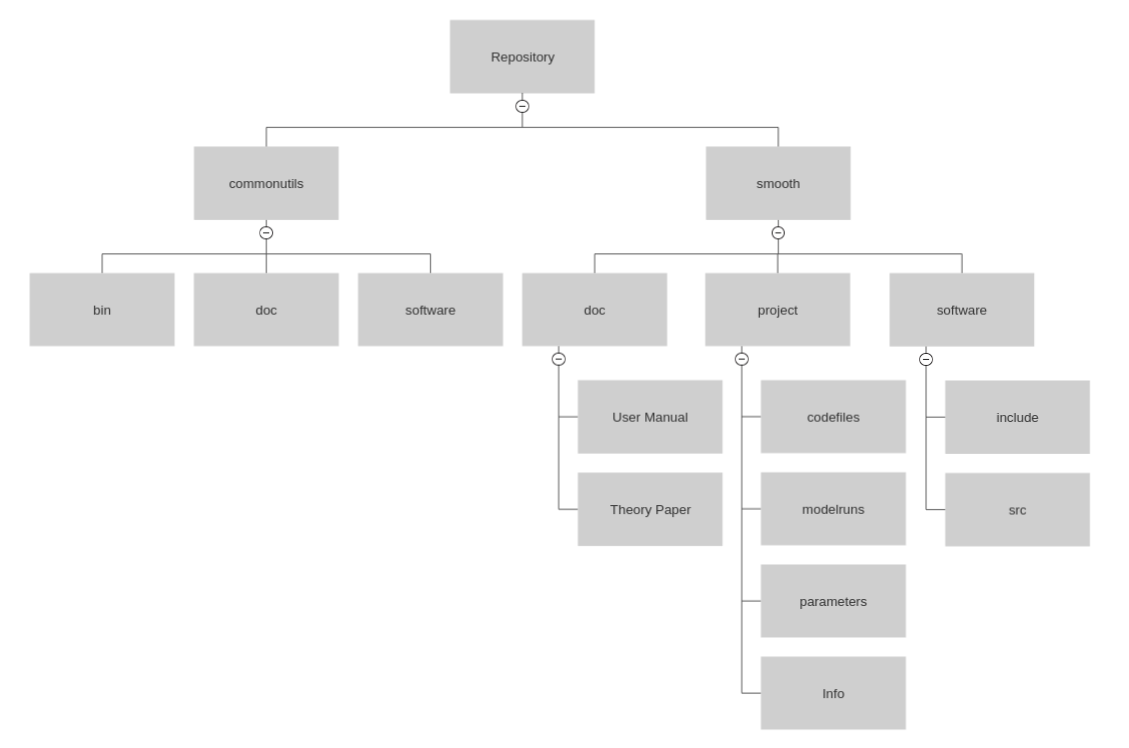
\includegraphics[width = 0.95\textwidth]{Structure_Tree.png}}

Once compiled, the libraries in the {\tt commonutils/} directory are used for a variety of tasks. These libaries are not particularly designed for {\it Smooth Emulator} or {\it Simplex Sampler}. The {\tt smooth/} directory contains codes that are used to create libraries specific to the sampler and emulator. The Executables are stored in {\tt smooth/local/bin}. The short main program source files are located in {\tt smooth/local/main\_programs/}. It is not envisioned that the User would edit files in the {\tt smooth/software/} directory, but that the User may well wish to create custom versions of the short main programs in {\tt smooth/local/main\_programs/}.

\subsection{Compiling Libraries }

First, change into software directories, then create the makefiles with cmake, then compile them.\\
\vspace{-20pt}
{\tt 
\begin{verbatim}
    % cd GITHOME_MSU/commonutils/software
    GITHOME_MSU/commonutils/software% cmake .
    GITHOME_MSU/commonutils/software% make
    GITHOME_MSU/commonutils/software% cd ../GITHOME_MSU/smooth/software
    GITHOME_MSU/smooth/software% cmake .
    GITHOME_MSU/smooth/software% make
\end{verbatim}
At this point all the libraries are built, but this does not include the main programs. The main programs, are short, and are located in a separate location, as they are meant to serve as examples which the User might copy and edit at will.

Finally, compile the main programs. Below, this illustrates how to build the programs used for generating training points with Simplex and for tuning the emulator with Smoothy:
\begin{verbatim}
    % cd MY_LOCAL/build
    MY_LOCAL/build% cmake .
    MY_LOCAL/build% make simplex
    MY_LOCAL/build% make smoothy_tune
    .
    .
\end{verbatim}
}
Other source codes for main programs can be found in {\tt MY\_LOCAL/main\_programs/}. If you build your own main programs (probably using these as examples), you can edit the {\tt CMakeList.txt} file in {\tt GITHOME\_MSU/smooth/local/build}, using the existing entries as an example. The executables should appear in {\tt MY\_LOCAL/bin/}. 

\subsection{The Project Directory}

Within {\tt MY\_PROJECT/} there are three sub-directories (assuming it was created from the template). The first is {\tt MY\_PROJECT/Info/}. Information about the model parameters, and their priors is stored in {\tt MY\_PROJECT/prior\_info.txt}, and information about the observables is store in {\tt MY\_PROJECT/observable\_info.txt}. The {\tt MY\_PROJECT/parameters} directory stores user-defined parameter files used by {\it Simplex Sampler}, {\tt MY\_PROJECT/parameters/simplex\_parameters.txt}, and by {\it Smooth Emulator} {\tt MY\_PROJECT/parameters/emulator\_parameters.txt}. The {\tt MY\_PROJECT/modelruns} directory will store information for each full-model run. The directories {\tt  MY\_PROJECT/modelruns/run0/}, {\tt  MY\_PROJECT/modelruns/run1/}, $\cdots$, have files describing the model parameters for each run, along with the output required by the emulator for each specific full-model run. For example, the {\tt  MY\_PROJECT/modelruns/run1/} directory has the files {\tt mod\_parameters.txt} and {\tt obs.txt}. The first file stores the model parameter values for that particular training run. The User then runs their full model based on those parameters and stores the corresponding observables in {\tt obs.txt}. The User may generate the {\tt mod\_parameters.txt} files using {\it Simplex Sampler}, or the user might generate them according to some other prescription. Once the User has then generated the {\tt obs.txt} files, {\it Smooth Emulator} can then build and tune the emulator.

\end{document}
